%%%
%%% AlbLaTeX/doc/user/alb-float-tools.tex
%%%
%%%     See copyright notice, and license in text.
%%%
%%%   - Documentation for the 'alb-float-tools' LaTeX package.
%%%



\documentclass[11pt,a4paper,oneside,titlepage]{alb-latex}



%
% URL Typesetting
%
% See: 'url.sty'.

\usepackage{url}


%
% Encapsulated postscript/PDF handling.
%
% See: 'grfguide.ps' and 'pfgguide.ps'.

\usepackage{graphicx}


%
% The package being documented.

\usepackage{alb-float-tools}


%
% Sloppy Line Breaks
%
% Turn off careful line breaks and hyphenation.

\sloppy



\begin{document}



%%%
%%% TITLE
%%%

\albTitle{%
  Typesetting Figures under \LaTeX{}%
}

\begin{albTitlePage}

  \albTitlePageSection{Author}

  Andrew Lincoln Burrow\\
  \url{albcorp@gmail.com}


  \albTitlePageSection{Abstract}

  The \texttt{AlbFloatTools} package provides a single
  \texttt{alb-float-tools} \LaTeX{} package to provide greater control
  over the layout of material in floats.  It is tailored to the
  typesetting of mathematical figures.  While the standard
  \texttt{figure} environment already supplies basic support, the
  package allows figure floats to extend into the document margins, and
  provides a mechanism to layout subfigures.  The package is supported
  by an emacs lisp file customising \AUCTeX{} and \RefTeX{} which
  automates the markup process of figure floats, graphic inclusions, and
  \texttt{psfrag} rewriting, and also constructs labels in the file
  namespace.  These extensions to \AUCTeX{} override the builtin support
  for the \texttt{graphicx} and \texttt{psfrag} packages.


  \albTitlePageSection{Copyright}

  Copyright \copyright{} 2001--2006, 2013 Andrew Lincoln Burrow.\\
  This program may be distributed and/or modified under the conditions
  of the \LaTeX{} Project Public License, either version 1.3 of this
  license or (at your option) any later version.

  \medskip{}

  The latest version of this license is in
  \begin{quote}
    \url{http://www.latex-project.org/lppl.txt}
  \end{quote}
  and version 1.3 or later is part of all distributions of LaTeX version
  2005/12/01 or later.

  \medskip{}

  This work has the LPPL maintenance status `author-maintained'.

  \medskip{}

  This work consists of the files
  \begin{quote}
    \begin{flushleft}
      \url{alb-algorithms.sty}, \url{alb-avm.sty}, \url{alb-latex.cls},
      \url{alb-float-tools.sty}, \url{alb-graph-theory.sty},
      \url{alb-journal.cls}, \url{alb-order-theory.sty},
      \url{alb-proofs.sty}, \url{alb-theorems.sty},
      \url{alb-thesis.cls}, \url{alb-algorithms.tex}, \url{alb-avm.tex},
      \url{alb-latex.tex}, \url{alb-float-tools.tex},
      \url{alb-graph-theory.tex}, \url{alb-journal.tex},
      \url{alb-order-theory.tex}, \url{alb-proofs.tex},
      \url{alb-theorems.tex}, \url{alb-thesis.tex}.
      \url{alb-journal-glossary.ist}, \url{alb-journal-index.ist},
      \url{alb-thesis-glossary.ist}, and \url{alb-thesis-index.ist}.
    \end{flushleft}
  \end{quote}


  \albTitlePageSection{Version Information}

  \verb$Revision$\\
  \verb$Date$

\end{albTitlePage}



%%%
%%% INTRODUCTION
%%%

\section{Introduction}
\label{sec:alb-float-tools-documentation:intr}

The \texttt{alb-float-tools} \LaTeX{} package is designed to extend the
standard figures and the support provided by \AUCTeX{} for both figures
and graphics.  The new \LaTeX{} features allow figures to utilise the
horizontal margin par allocations, and group subfigures.  The \AUCTeX{}
extensions prompting for these new features, and override
\texttt{graphicx.el} and \texttt{psfrag.el} to improve the prompting for
graphics inclusion and label rewriting.



%%%
%%% USING THE COMMANDS AND ENVIRONMENTS
%%%

\section{Using the Commands and Environments}
\label{sec:alb-float-tools-documentation:using-comm-envir}

The environments of \texttt{alb-float-tools} place certain syntactic
restrictions on their use.  This section concerns these restrictions and
the typographic meaning of the markup.
Section~\ref{sec:alb-float-tools-documentation:auctex-cust} describes
how the \AUCTeX{} customisation eases the burden of entering
syntactically correct \LaTeX{} code.


\subsection{Wide Figures}
\label{sec:alb-float-tools-documentation:wide-figures}

The \texttt{alb-float-tools} \LaTeX{} package provides the
\texttt{albInflate} environment for use within a float environment such
as \texttt{figure}.  The environment allows float material to extend
into the margin.  It is designed to work in any combination of oneside,
twoside, and reverse margin options, and also tests for case where the
figure occurs within a column.

\begin{description}
\item[\albLtxEnv{albInflate}\albLtxArg{label}] Inflate the column to
  include the marginpar allocation, where the marginpar location is
  calculated from the page reference of \albLtxPrm{label}.  This
  environment should only be used inside a float with a label, and the
  label of the float and the environment must match!

  For example,
  \begin{quote}
\begin{verbatim}
\begin{figure}
  \begin{albInflate}{fig:example-wide-figure}
    \centering
    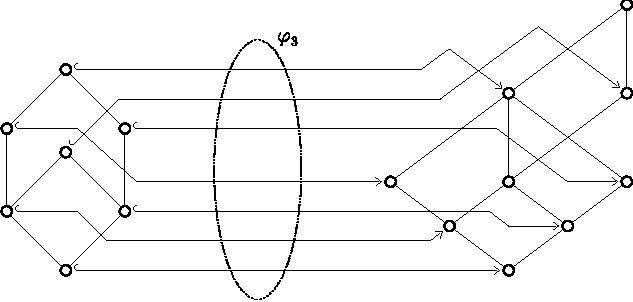
\includegraphics[scale=1.44]{poset-mapto-lattice.pdf}
  \end{albInflate}
  \caption[Example wide figure]{%
    An example of a wide figure.}
  \label{fig:example-wide-figure}
\end{figure}
\end{verbatim}
  \end{quote}
  produces Figure~\ref{fig:example-wide-figure}.

  \begin{figure}
    \begin{albInflate}{fig:example-wide-figure}
      \centering
      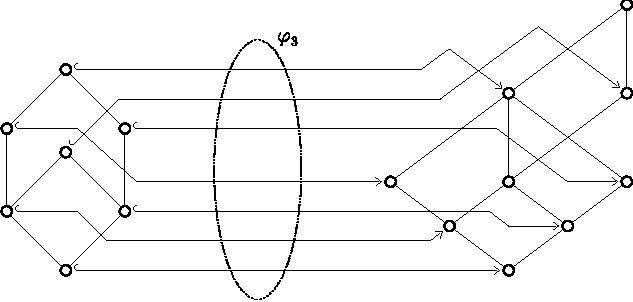
\includegraphics[scale=1.44]{poset-mapto-lattice.pdf}
    \end{albInflate}
    \caption[Example wide figure]{%
      An example of a wide figure.}
    \label{fig:example-wide-figure}
  \end{figure}

  The definition is easy in \texttt{oneside} mode, but requires cunning
  in \texttt{twoside} mode.  We must guess the final position of the
  float to decide which text edge to cross.  The solution is to look at
  the page number cross reference.  If the float was set on an odd page
  last run, then format for an odd page in this run.  LaTeX will still
  converge because only vertical size affects page layout.  Furthermore,
  it requires exactly the same number of LaTeX runs to converge, as the
  cross reference itself requires.
\end{description}


\subsection{Collections of Subfigures}
\label{sec:alb-float-tools-documentation:coll-subf}

The \texttt{alb-float-tools} package provides the \texttt{albShelve}
environment for use within a float environment such as \texttt{figure}.
The environment collects and labels subfigures.  The elements are
distributed across the available width, and flow onto additional lines
where required.  An optional argument controls whether the elements are
top-aligned or bottom-aligned.

\begin{description}
\item[\albLtxEnv{albShelve}\albLtxOpt{align}] Collect smaller figures
  within a larger figure.  This is a list environment in which the
  \albLtxCmd{item}\albLtxOpt{label} command marks-up subfigures with the
  optional tag \albLtxPrm{label}.  However, the list does not use a
  counter so that it does not enumerate or support the \albLtxCmd{label}
  command.  The list displays the subfigures across the column with each
  line of subfigures evenly spread across the space.  If
  \albLtxPrm{align} is \texttt{t} then the elements are top-aligned, and
  if \albLtxPrm{align} is \texttt{b} then the elements are
  bottom-aligned

  For example,
  \begin{quote}
\begin{verbatim}
\begin{figure}
  \begin{albShelve}[b]
  \item[(a)] 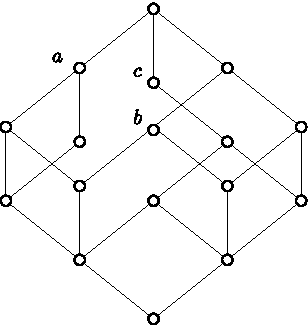
\includegraphics{down-closure-source.pdf}
  \item[(b)] 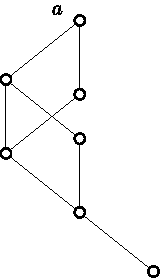
\includegraphics{down-closure-of-a.pdf}
  \item[(c)] 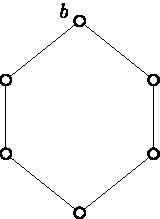
\includegraphics{down-closure-of-b.pdf}
  \item[(d)] 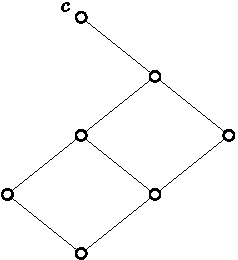
\includegraphics{down-closure-of-c.pdf}
  \end{albShelve}
  \caption[Example subfigure collection]{%
    An example of a subfigure collection.}
  \label{fig:example-subf-coll}
\end{figure}
\end{verbatim}
  \end{quote}
  produces Figure~\ref{fig:example-subf-coll}.

  \begin{figure}[!t]
    \begin{albShelve}[b]
    \item[(a)] 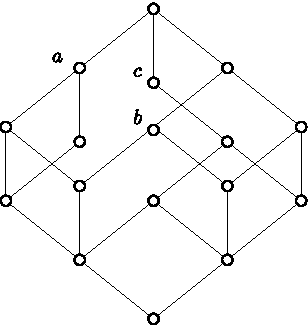
\includegraphics{down-closure-source.pdf}
    \item[(b)] 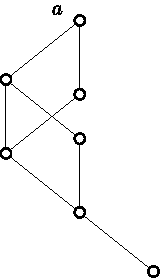
\includegraphics{down-closure-of-a.pdf}
    \item[(c)] 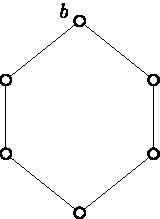
\includegraphics{down-closure-of-b.pdf}
    \item[(d)] 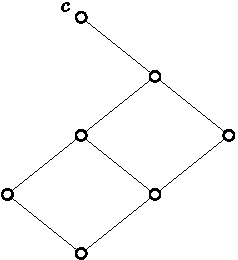
\includegraphics{down-closure-of-c.pdf}
    \end{albShelve}
    \caption[Example subfigure collection]{%
      An example of a subfigure collection.}
    \label{fig:example-subf-coll}
  \end{figure}
\end{description}



%%%
%%% AUCTEX CUSTOMISATIONS
%%%

\section{\AUCTeX\ Customisations}
\label{sec:alb-float-tools-documentation:auctex-cust}

Under \AUCTeX{} the file \texttt{alb-float-tools.el} is automatically
loaded whenever the \texttt{alb-float-tools} package is used.  The
customisation adds support for the symbols and environments from
\texttt{alb-float-tools}.  In addition, the \AUCTeX{} supplied
customisations for \texttt{graphicx} and \texttt{psfrag} are overridden.
This results in the following improved prompting.

\begin{description}
\item[\texttt{figure}] Prompts and constructs the float environment.
  The prompts follow the following sequence.

  \begin{description}
  \item[(optional) Float to] Complete to one of the \LaTeX{} locations
    \texttt{h}, \texttt{t}, \texttt{b}, or \texttt{p}.

  \item[(optional) Abbreviated caption:] The abbreviated caption is used
    in the list of figures, and to generate a label for the figure.  It
    is best to have a well planned one line description ready before
    inserting a figure.

  \item[Caption:] If you provide an abbreviated caption, then this
    starts as the abbreviated caption.  You can expand it now, or later
    because the label will be derived from the abbreviated caption.

  \item[Label:] If you provide an abbreviated caption, then this is
    already generated for you.  Otherwise, you will need to provide a
    label.  It is required for the inflate option.
  \end{description}

\item[\texttt{albInflate}] Constructs the inflate environment inside a
  float environment, and searches within the enclosing environment for a
  label to use to compute the margin crossing.

\item[\texttt{albShelve}] Constructs the shelve environment inside a
  float environment, and prompts for the alignment of the elements.

\item[\texttt{includegraphics}] Constructs the \texttt{includegraphics}
  command, and prompts for options, and the local graphics files.

\item[\texttt{psfrags}] Constructs the \texttt{psfrags} environment and
  a list of \texttt{psfrag} command tag replacements.  While the user
  inputs non-empty tags, \AUCTeX{} prompts for the components of a
  \texttt{psfrag} command.
\end{description}



%%%
%%% MAKEFILE TARGETS
%%%

\section{Makefile Targets}
\label{sec:alb-float-tools:makef-targ}

The inclusion of graphic files affects document compilation, since
graphic files must often be converted into an appropriate format.  This
in turn affects the choice of markup.  The makefile from the
\texttt{AlbLaTeXDocumentTemplate} package, attempts to automate the
graphic file transformations for \PDFLaTeX{} compilation.  In this case,
the \texttt{includegraphics} command accepts PDF, JPEG, and PNG
graphics.  The makefile attempts to construct these formats from other
source formats such as SVG.  Therefore, each filename should include the
extension to assist in the search for possible transformations.



\end{document}



%%% Local Variables:
%%% mode: latex
%%% TeX-master: t
%%% ispell-local-dictionary: "british"
%%% End:
